\begin{figure}[h!]
    \centering
    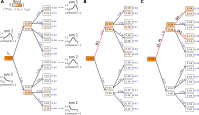
\includegraphics[width=1\textwidth]{Figures/supp/supp1.png}
    \caption{\textbf{Replay updates in Bandit belief space.} A) Planning tree of horizon $2$ constructed by the subject. Each rectangle corresponds to a distinct belief state. The leftmost belief state corresponds to the subject's prior belief, $b_\rho$, at which the tree is rooted. The insets next to some belief states graphically demonstrate the subject's belief about the payoff of one of the arms in those belief states (the red dotted lines show the expected payoffs). For the paired belief states, the top ones always result from imagined successful outcomes (received a reward of $1$), whereas the bottoms ones -- from imagined failed outcomes (received a reward of $0$). Belief states are coloured according to the Need at those belief states calculated by the subject; moreover, Need is additionally shown with numbers in each belief state. Since the subject's behavioural policy is stochastic (softmax), all belief states have positive estimated Need (for some belief states, Need was rounded up to two decimal places). The black arrows show actions available at each belief state. The top arrows always denote the choice of arm $1$ and the bottom ones -- arm $2$. The blue numbers above each action arrow denote the $Q$-values associated with each action in every belief state. B) Single replay update in the belief tree. The subject chose to update the $Q$-value of arm $1$ at the prior belief state (the updated action arrow is highlighted in red) towards the expected value of the two belief states at the next horizon (the new updated value is highlighted in red). This replay update was executed because i) it was estimated to have the greatest EVB; and ii) the estimated EVB of this update exceeded the EVB threshold. Note the effect of generalisation of this individual replay update which is visible in how the Need that the subject calculates for all other belief states changes throughout the tree. C) All replay updates executed by the subject until the estimated benefit was calculated to be below the EVB threshold. The bold numbers in squared brackets show the order in which those updates were executed.}
    \label{fig:supp1}
\end{figure}

\begin{figure}[h!]
    \centering
    \includegraphics[width=1\textwidth]{Figures/supp/supp2.png}
    \caption{\textbf{Policy improvement occasioned by replay.} Top: Evolution of the value of the root belief state (same as in Fig~\ref{fig:supp1}) due to replay as a function of the EVB threhsold, $\xi$. Middle: Evolution of the value of the policy (evaluated in the belief tree) which resulted from replay updates at different EVB thresholds. Bottom: Total number of replay updates executed for the different EVB thresholds.}
    \label{fig:supp2}
\end{figure}

\begin{figure}[h!]
    \centering
    \includegraphics[width=0.9\textwidth]{Figures/supp/supp3.png}
    \caption{\textbf{Effect of initialised behavioural policy}. Top: The final value of the root belief state (same as in Fig~\ref{fig:supp1}) due to replay with a fixed EVB threshold. The initialised values of all belief states were randomised to imitate noisy initial experience (or potential changes in the bandit payoff probabilities). The bars show average root belief state values over $100$ different tree initialisations. Each dot corresponds to an individual tree. Bottom: Same as above but for the value of the updated policy evaluated in the tree.}
    \label{fig:supp3}
\end{figure}

\begin{figure}[h!]
    \centering
    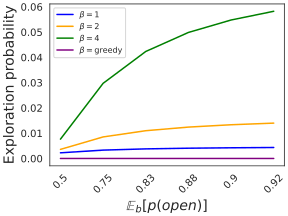
\includegraphics[width=0.9\textwidth]{Figures/supp/supp4.png}
    \caption{\textbf{Sequence replay statistics}. Left: Proportion of forward to reverse sequences replayed in the belief tree with the same prior belief as in Fig~\ref{fig:supp1} with planning horizon set to $4$. The initialised values of all belief states were randomised as in Fig~\ref{fig:supp3}. The bar shows average proportion over $100$ different tree initialisations. Right: Average number of replayed actions in the same tree initialisations as above with and without sequence replay.}
    \label{fig:supp4}
\end{figure}

\begin{figure}[h!]
    \centering
    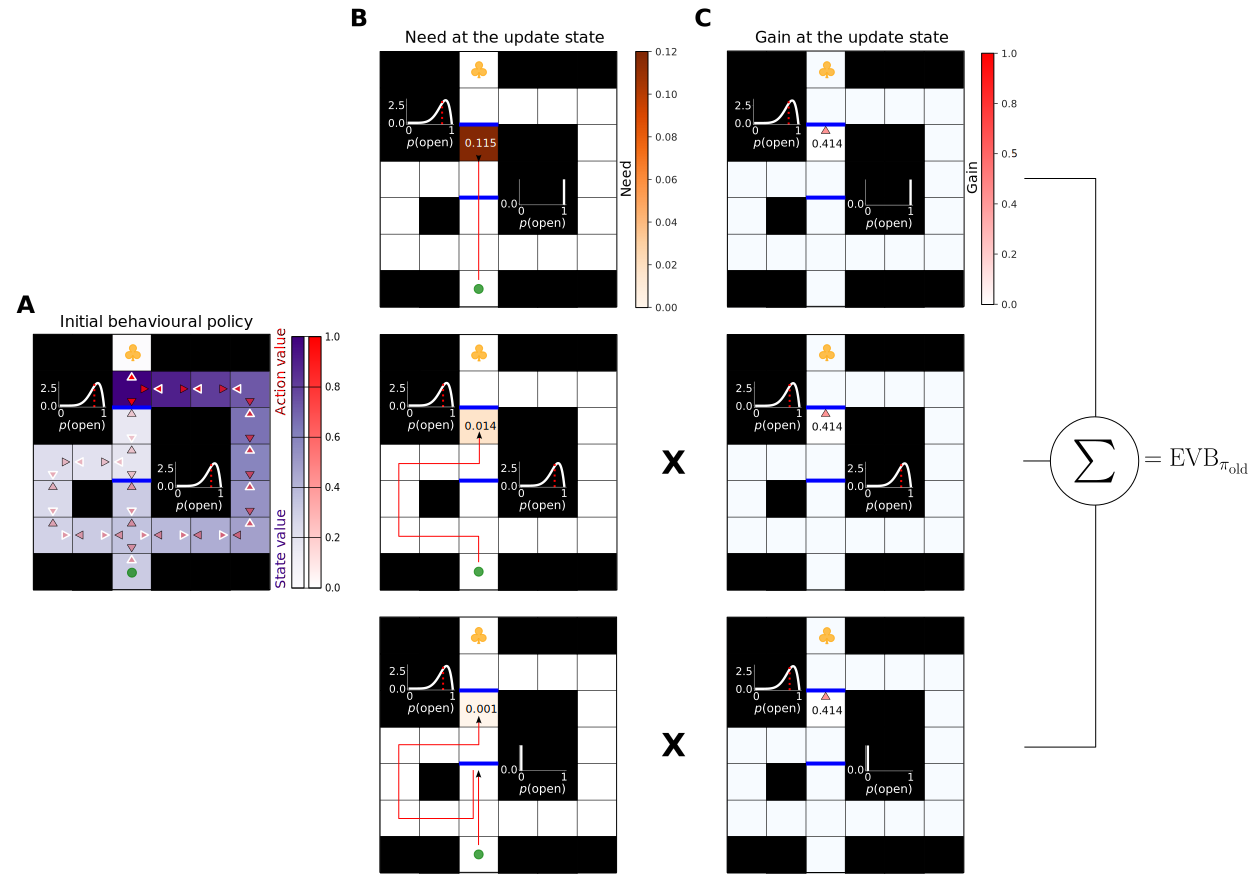
\includegraphics[width=1\textwidth]{Figures/supp/supp5.png}
    \caption{\textbf{Uncertainty affects replay choices and their behavioural readout.} The layout of the figure is similar to that of Fig~\ref{fig:fig3}. A) In this instance, however, the subject's belief was more pessimistic since it indicated a lower chance of the top barrier being potentially open. B) The value of exploration was estimated to be lower, and therefore it did not propagate deep enough (towards the subject's location). C) The updated policy still prescribed the subject to exploit the longer path, since the critical action at the junction between the different arms had not been updated by exploratory replay.}
    \label{fig:supp5}
\end{figure}

\begin{figure}[h!]
    \centering
    \includegraphics[width=0.5\textwidth]{Figures/supp/supp6.png}
    \caption{\textbf{Relationship between uncertainty, behavioural policy and exploration quality.} The graph shows the marginal probability of directed exploration (approaching and attempting the potential barrier in Figs~\ref{fig:fig2} and~\ref{fig:fig3} from the start state) as a function of the subject's uncertainty and the greediness of its behavioural policy. As the subject's belief in the absence of the barrier increased, it became progressively more likely to engage in the act of directed exploration. The same softmax policy with inverse temperature $\beta=2$ was used to calculate the priority of replay updates. However, applying different inverse temperature parameters (which subjects might heuristically use to arrange for offline exploration) to the resulting exploratory value function yielded policies with different incentives for exploration.}
    \label{fig:supp6}
\end{figure}